% Created 2023-01-06 Sex 15:04
% Intended LaTeX compiler: pdflatex
\documentclass[a4paper]{article}
\usepackage[utf8]{inputenc}
\usepackage[T1]{fontenc}
\usepackage{graphicx}
\usepackage{longtable}
\usepackage{wrapfig}
\usepackage{rotating}
\usepackage[normalem]{ulem}
\usepackage{amsmath}
\usepackage{amssymb}
\usepackage{capt-of}
\usepackage{hyperref}
\usepackage{nopageno}
\usepackage{pdfpages}
\author{Davi Raubach}
\date{}
\title{omcwb}
\hypersetup{
 pdfauthor={Davi Raubach},
 pdftitle={omcwb},
 pdfkeywords={},
 pdfsubject={},
 pdfcreator={Emacs 29.0.50 (Org mode 9.5.4)}, 
 pdflang={English}}
\begin{document}

\maketitle



\section*{Prefácio}
\label{sec:org2d2effd}
Nesta composição, a leitura de um texto verbal ocupa uma posição de geração de material musical e de organizador relativo da temporalidade. Em boa parte da peça, o passar do tempo é articulado pela leitura do texto.

O poema abaixo cumpre essa função na peça foi escrito para essa ocasião.

Palavra atirada contra a água \\
Salta, salta, voa\\
Pousa sobre as nuvens\\
Mergulha cada vez mais fundo\\
Cada vez mais alto\\
Seduz a língua e escoa\\
Escoa, salta, voa\\
Cada vez mais sonhada

\textbf{Duração} c. 4 min

\section*{Notas de Performance}
\label{sec:org9440280}

\subsection*{Notação rítmica}
\label{sec:org1b02727}

\textbf{Tempo Estrito}: Notado tradicionalmente
\textbf{Tempo de fala}: Gestos instrumentais estão associados às sílabas do texto. O/A intérprete deve executar a música levando em conta sua associação com o texto. Uma leitura mental é que determina quando tocar. Pontos e vírgulas podem ser interpretados como pausas, fraseseado e dinâmicas podem derivar também do texto.

Cabeça de nota como de semínima representa a leitura de uma sílaba para cada nota (notas mais curtas). Cabeça de nota como de mínimas representam notas que se estendem por várias sílabas (notas mais longas):

\begin{center}
\includesvg[width=.9\linewidth]{exemplo_tempo_fala}
\end{center}

Em geral, o ritmo instrumental deve se submeter ao ritmo da leitura. Entretanto, também deve-se levar em consideração que alguns gestos precisam de tempo hábil para a exeucução e nestes casos não há problema em suspender o tempo da leitura.



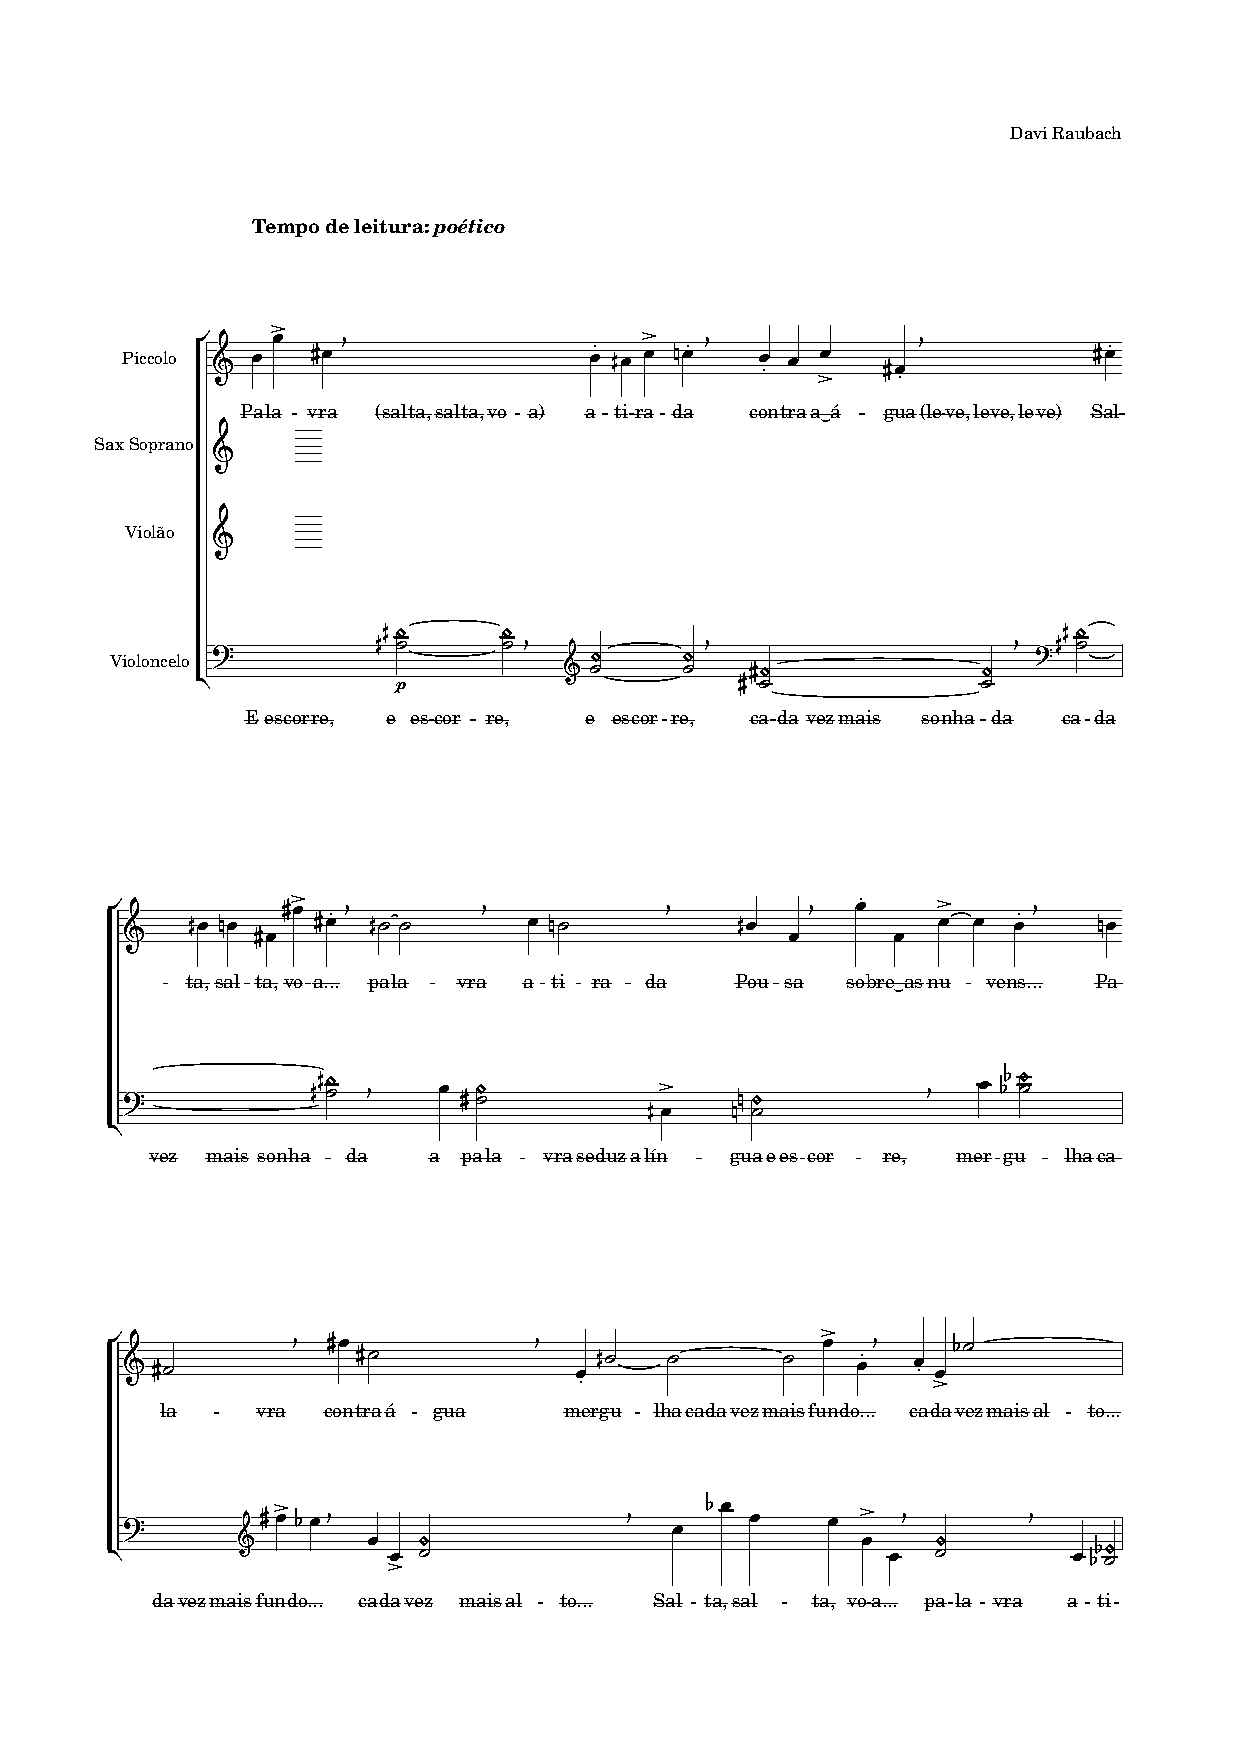
\includepdf[pages=-,pagecommand={}]{score_org.pdf}
\end{document}